\documentclass[11pt,a4paper]{article}
\usepackage[french]{babel}
\usepackage[T1]{fontenc}
\usepackage[utf8]{inputenc}
\usepackage{graphicx}
\usepackage{color}
\usepackage{hyperref}
\usepackage{glossaries}

\makeglossaries

\newglossaryentry{degats}
{
    name=dégâts,
    description={Quantité de points de vie retirés au monstre}
}
\newglossaryentry{amelioration}
{
    name=amélioration,
    description={Augmentation des dégâts du joueur ou des héros}
}
\newglossaryentry{or}
{
    name=or,
    description={Monnaie du jeu, obligatoire pour les améliorations}
}
\newglossaryentry{prestige}
{
    name=prestige,
    description={recommencé le jeu mais avec des points à dépenser dans un arbre de compétences.}
}
\newglossaryentry{hors ligne}
{
    name=hors ligne,
    description={Le joueur n'a pas le jeu ouvert mais le jeu continue de tourner}
}
\newglossaryentry{temps de recharge}
{
    name=temps de recharge,
    description={Le joueur doit attendre un certain temps avant de pouvoir recommencer un challenge}
}
\newglossaryentry{challenge}
{
    name=challenge,
    description={Un défi que le joueur doit relever pour gagner des récompenses}
}

\begin{document}    

\begin{figure}[t]
    
\includegraphics[width=4cm]{img/logolemansU.png}\hfill
    
\includegraphics[width=4cm]{img/logo_IC2.png}\\
\end{figure}
\title{\textcolor{blue}{\textbf{Le Mans Université}}\\
Licence Informatique 2\up{e} année\\
Module 174UP02 Rapport de Projet\\
\textbf{TapVenture}}
\author{Noam MANFALOTI, Ibrahim SAPIEV, Lucas DUPONT et Logan Evenisse}
\date{\today}
\maketitle
\begin{center}
    \href{https://github.com/nmanfaloti/TapVenture}{\textcolor{blue}{Lien du projet}}
\end{center}
\newpage
\tableofcontents
\newpage

\section{Introduction}
L'objet de ce document est de présenter le projet de développement du jeu TapVenture réalisé dans le cadre du module Conduite de Projet L2 Informatique de Le Mans Université sur une 
période de janvier à avril 2025. Le jeu TapVenture a été réalisé en langage C et avec la bibliothèque graphique SDL.\\
Le jeu TapVenture se base sur un concept de clic (catégorie de jeu de type \href{https://en.wikipedia.org/wiki/Incremental_game}{\textcolor{blue}{Clicker}}). 
Le joueur doit cliquer sur des monstres pour gagner de l'\gls{or} et améliorer les \gls{degats} afin de gagner plus d'or. Ensuite, le joueur peut acheter des héros qui vont 
combattre les monstres automatiquement. Et lorsqu'il atteint le dernier niveau, il <<prestige>>, c'est-à-dire qu'il recommence le jeu mais avec des points à 
dépenser dans un arbre de compétences.\\
Nous verrons dans une première partie la présentation du jeu et de ses principales fonctionnalités. Les éléments de gestion de projet feront l'objet d'une deuxième partie. 
Dans une troisième partie, nous décrirons les étapes de conception et de réalisation avant de conclure sur les aspects positifs et les limites de notre projet.
\\
\section{Analyse et conception}

\subsection{Description du projet}
Le joueur commence l'aventure en cliquant sur les monstres pour les vaincre et récupérer leur or. Cet or sert ensuite à recruter de nouveaux héros qui attaquent à la place du joueur et à
augmenter les dégâts que le joueur et ses héros infligent, permettant ainsi une progression exponentielle de la puissance de l'utilisateur.
Le gameplay repose sur une boucle addictive d’accomplissement de tâches, de gain d'or, et d’\gls{amelioration} de ses moyens d’attaque.
La progression se déroule à travers plusieurs niveaux, chacun situé dans un univers aux défis et aux monstres croissants. Pour passer au niveau suivant, le joueur doit vaincre 10 fois
les monstres de l’étape. Tous les 5 niveaux, un boss apparaît et doit être vaincu dans un temps imparti. À l’issue du dernier monde, le joueur <<\gls{prestige}>>.
Enfin, TapVenture intègre des fonctionnalités complémentaires telles qu’un système multilingue, des \gls{challenge}, ainsi qu’un système de récompense \gls{hors ligne}. La gestion de la
sauvegarde permet de reprendre le jeu quand on le souhaite, pour une expérience utilisateur optimale.


\subsection{Fonctionnalités}
Notre projet, TapVenture, intègre plusieurs fonctionnalités clés. Voici les fonctionnalités développées:
\begin{itemize}
    \item \textbf{Système de combat}: Un mécanisme interactif permettant aux joueurs d'affronter des ennemis et de progresser dans le jeu.
    \item \textbf{Système de progression}: Les joueurs peuvent améliorer leurs dégâts et leurs héros au fil du temps, offrant une expérience de jeu évolutive, Lorsqu'ils atteignent le dernier niveau, ils doivent vaincre le boss final pour effectuer un prestige.
    \item \textbf{Système d' or}: Une monnaie virtuelle qui est utilisée pour acheter des améliorations et des héros dans le jeu.
    \item \textbf{Système de magasin}: Une boutique qui permet aux joueurs d'acquérir de nouveaux héros et d'augmenter ses dégâts.
    \item \textbf{Système de défis}: Des défis disponibles toutes les 30 minutes pour gagner des récompenses supplémentaires.
    \item \textbf{Système de langue}: Le jeu est multilingue, permettant aux utilisateurs de choisir leur langue préférée.
    \item \textbf{Arbre de compétences (prestige)}: Un système d'arbre de compétences permet aux joueurs de débloquer des améliorations passives en échange de points de prestige.
        Il est composé de 3 branches, chacune ayant un thème spécifique.
        La branche d'or augmente les gains d'or du joueur, la branche de dégâts augmente les dégâts infligés, et la branche de prestige augmente les points de prestige gagnés par le joueur, ainsi que les héros gardés lors du prestige.
    \item \textbf{Système de sauvegarde}: Les progrès des joueurs sont sauvegardés automatiquement, garantissant une continuité de l'expérience de jeu.
    \item \textbf{Système de récompenses hors ligne}: Les joueurs reçoivent des récompenses même lorsqu'ils ne sont pas connectés, favorisant une progression continue.
    \item \textbf{Système d'inventaire et de scroll}: Un système d'inventaire qui permet aux joueurs de gérer leurs objets et de faire défiler les éléments de manière fluide.
    \item \textbf{Système de notification}: Un système de notification qui informe les joueurs des événements importants, tels que la fin d'un défi ou l'arrivée d'un nouveau monstre.
\end{itemize}
\subsection{Direction artistique}
La direction artistique de TapVenture s'inspire d'un style fantastique moderne, combinant des éléments visuels immersifs et dynamiques. 
Afin de pouvoir offrir aux utilisateurs une expérience de jeu engageante et attrayante, nous avons opté pour des graphismes colorés, avec des animations pour rendre le jeu plus vivant et interactif.
\section{Gestion du projet}
Cette partie présente la planification du projet, l'organisation du travail au début et tout au long des séances, ainsi que les outils de travail utilisés pour assurer une collaboration efficace.

\subsection{Planification}
Au début du projet, nous avons établi un diagramme de Gantt prévisionnel \footnote{Voir le Gantt prévisionnel: \href{https://docs.google.com/spreadsheets/d/1jvVkITa50-fjbtQPN5y54wZTgIkTPtt-_RPIWB4DkVM/edit?usp=sharing}{\textcolor{blue}{Gantt prévisionnel}}} pour planifier les différentes étapes du développement. Ce diagramme nous a permis de:
\begin{itemize}
    \item Définir et répartir les tâches sur la période de janvier à avril.
    \item Définir des jalons importants, tels que la fin de la conception, le début des tests et la livraison finale.
    \item Identifier les dépendances entre les tâches pour éviter les blocages.
    \item Prioriser les étapes critiques afin de garantir une progression fluide.
\end{itemize}
Le diagramme de Gantt prévisionnel a été conçu pour refléter les grandes étapes suivantes:
\begin{enumerate}
    \item \textbf{Initialisation}: 
    \begin{itemize}
        \item Formation à SDL.
        \item Mise en place de l'environnement technique.
        \item Réflexion sur l'optimisation du jeu.
        \item Analyse de la mécanique de jeu.
        \item Création du planning global du projet.
        \item Préparation de l’environnement de développement.
    \end{itemize}
    \item \textbf{Conception}: 
    \begin{itemize}
        \item Conception de l'UI.
        \item Choix du style graphique.
        \item Définition de la progression du jeu.
        \item Définition des mécaniques de jeu.
    \end{itemize}
    \item \textbf{Codage \& Test}:
    \begin{itemize}
        \item Développement des mécaniques de base.
        \item Création des premiers assets graphiques.
        \item Programmation du gameplay.
        \item Tests internes pour identifier les bugs et vérifier la stabilité.
        \item Ajustements après tests et optimisation des performances.
    \end{itemize}
    \item \textbf{Finalisation}: 
    \begin{itemize}
        \item Corrections finales des bugs.
        \item Optimisation du code et des assets graphiques.
        \item Préparation de la version finale pour livraison.
    \end{itemize}
    \item \textbf{Livraison}: 
    \begin{itemize}
        \item Rédaction du rapport.
        \item Préparation de la soutenance.
    \end{itemize}
\end{enumerate}

\subsection{Organisation du travail}
Pour organiser le travail, nous avons adopté une approche collaborative et structurée:
\begin{itemize}
    \item \textbf{Répartition des tâches}: Des tâches précise ont été attribuées en fonction des compétences et des préférences de chaque membre de l'équipe. Par exemple, certains se sont concentrés sur le développement des fonctionnalités principales, tandis que d'autres ont travaillé sur l'interface utilisateur ou les tests.
    \item \textbf{Réunions régulières}: Chaque séance de travail débutait par une réunion rapide pour faire le point sur l'avancement, discuter des éventuels problèmes rencontrés et ajuster les priorités si nécessaire.
    \item \textbf{Mise à jour du planning}: Le diagramme de Gantt et le tableau Kanban ont été mis à jour régulièrement pour refléter l'état réel du projet. Cela nous a permis de:
    \begin{itemize}
        \item Comparer le planning initial avec l'avancement réel.
        \item Identifier les écarts et ajuster les priorités en conséquence.
        \item Maintenir une vision claire des étapes restantes.
    \end{itemize}
\end{itemize}

\subsection{Outils de travail}
Pour faciliter la collaboration et assurer une bonne coordination, nous avons utilisé plusieurs outils adaptés à nos besoins:
\begin{itemize}
    \item \textbf{GitHub}: Utilisé pour le versionnement du code, le suivi des modifications. Cela a permis à chaque membre de travailler sur des fonctionnalités spécifiques et de voir les changement et mise a jour effectuer.
    \item \textbf{Discord}: Utilisé pour la communication en temps réel, les réunions à distance et le partage rapide d'informations. Cet outil a été particulièrement utile pour maintenir une bonne communication, même en dehors des séances de travail.
    \item \textbf{Outil Kanban}: Un tableau Kanban dans le git a été utilisé pour suivre l'avancement des tâches. Les colonnes représentaient les différentes étapes: todo (ce qui est a faire), in progress (le travail en cours), Done séance X (ce qui a été fait a la X\up{e} séance), et les cartes correspondaient aux tâches spécifiques. Cela nous a permis de visualiser facilement l'état d'avancement du projet.
\end{itemize}
Ces outils ont joué un rôle clé dans la réussite du projet en nous permettant de travailler efficacement, même à distance, et de maintenir une bonne coordination au sein de l'équipe.
\newpage
\section{Realisation}
Cette partie présente les différentes étapes de la réalisation du projet TapVenture, ainsi que les choix techniques effectués.
\subsection{Gestion des textes et de la traduction}
Le fichier \texttt{chaine.c} contient plusieurs fonctions dédiées à la manipulation dynamique des chaînes de caractères, permettant de construire, formater et traduire des textes de manière flexible.
La fonction \texttt{formatChaine} reprend le principe de la fonction \texttt{printf}. Son objectif n’est pas de produire un affichage mais de créer une chaîne de caractère et d'allouer le bon espace mémoire. Les paramètres de la fonction sont les même que \texttt{printf}, a l’exception que les seules types acceptés sont ceux que nous utilisons \texttt{int}, \texttt{float}, \texttt{string} et nos types personnalisée:

\begin{itemize}
    \item \texttt{\%w}: pour afficher un nombre de type unsigned long long int avec un format compact.
 	\item \texttt{\%t}: pour insérer une traduction via la fonction Traduction
\end{itemize}

Dans TapVenture, les nombres peuvent devenir extrêmement grands en fin de partie, c'est pourquoi nous utilisons des unsigned long long int. Mais leur affichage à l'écran est difficilement lisible pour le joueur au-delà de 4 chiffres. Pour résoudre ce problème, le format personnalisé \texttt{\%w} est utilisé, géré par la fonction \texttt{formatULLI}. Cette fonction prend en paramètre un unsigned long long int et renvoie une chaîne de caractères allouée dynamiquement, représentant le nombre dans un format plus compact. Par exemple, le nombre 1234 est transformé en 123A, a chaque dizaine supplémentaire la lettre de l'alphabet est incrémentée. Ce format d'affichage améliore considérablement la lisibilité des nombres pour le joueur.\\
La fonction \texttt{Traduction} présente dans le fichier \texttt{lang.c} prend en paramètre un enum \texttt{cleMsg} qui permet de représenter l’indice du texte dans un tableau de chaîne de caractère. Chaque langue a son propre tableau contenant toutes ses traductions. La fonction renvoie la chaîne dans le tableau de la langue actuelle.  

\subsection{Gestion de l'interface utilisateur}
Cette partie détaille la gestion de l'interface utilisateur, qui comporte les boutons, les textes, les images et les notifications.

\subsubsection{Structure de données} 
L'interface utilisateur est organisée autour de plusieurs structures clés:\\
\begin{itemize}
    \item \textbf{uiPage}: Représente une page complète de l'interface, contenant un conteneur pour les éléments d'interface, une liste de boutons et une liste de buttonImg.
    \item \textbf{pageHolder}: Structure globale qui stocke toutes les pages du jeu, permettant de naviguer entre elles.
    \item \textbf{uiContainer}: Contient les éléments d'interface d'une page (textes, images).
    \item \textbf{uiTxt}: Élément textuel de l'interface, caractérisé par son contenu, sa police, sa couleur et sa position.
    \item \textbf{uiImg}: Élément graphique de l'interface, défini par son chemin d'image, sa position et son identificateur.
    \item \textbf{Button}: Élément interactif permettant aux joueurs d'effectuer des actions, caractérisé par son texte, sa position, son apparence et la fonction qu'il déclenche lors d'un clic.
    \item \textbf{ButtonImg}: Un élément avec les mêmes caractéristiques que Button, mais qui utilise une image comme icône à la place du texte.
    \item \textbf{Notif}: Une notification qui s'affiche sur l'écran pendant un temps défini, elle est caractérisée par son titre, sa description, sa position, sa taille et son image de fond.
    \item \textbf{NotifList}: Une liste de notifications, qui contient un tableau de Notif et un compteur pour suivre le nombre de notifications affichées.
\end{itemize}
Dans chaque élément d’interface lié à SDL, nous avons sauvegardé les textures des éléments afin de ne pas les recréer a chaque fois. cette texture est donc détruite et recréer lors d'un changement d'apparence sur un bouton (sauf s’il s’agit d'un changement de texte).

\begin{figure}[h] 
    \begin{minipage}{0.48\textwidth} 
        \centering
        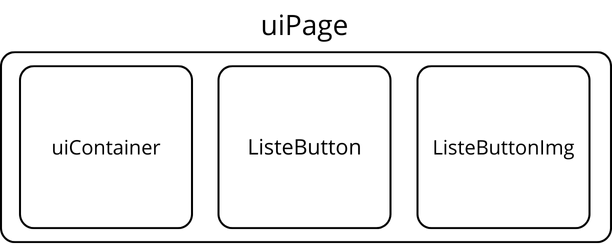
\includegraphics[width=\textwidth]{img/page_schema.png} 
        \caption{Structure d'uiPage} 
    \end{minipage} 
    \hfill 
    \begin{minipage}{0.48\textwidth} 
        \centering 
        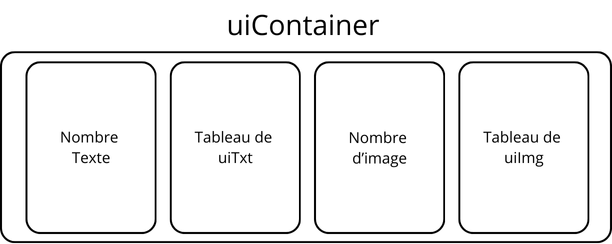
\includegraphics[width=\textwidth]{img/uiContainer_schema.png} 
        \caption{Structure d'uiContainer}
    \end{minipage} 
\end{figure}

\subsubsection{Fonctions de gestion de l'interface} 
\begin{itemize} 
    \item \texttt{createPage}: Initialise une nouvelle page en allouant la mémoire nécessaire pour son conteneur et en initialisant ses propriétés. La fonction prend en paramètre un pointeur vers la page à créer et ne renvoie rien.
    \item \texttt{destroyPage}: Libère la mémoire utilisée par une page, y compris tous ses éléments d'interface. Elle prend en paramètre un pointeur vers la page à détruire et ne renvoie rien.
    \item \texttt{createUIText}: Crée un élément textuel et l'ajoute à une page spécifique. Elle prend en paramètre la page cible, la police à utiliser, le texte à afficher, sa position, sa couleur et un identifiant.
    \item \texttt{createUIImg}: Ajoute une image à l'interface utilisateur. Elle prend en paramètre la page cible, le chemin de l'image, sa position et un identifiant.
    \item \texttt{createButton}: Crée un bouton interactif avec une apparence et une fonction spécifiques, ainsi qu'un coefficient de grossissement lors du hover de l'élément. Elle prend en paramètre la page cible, la position du bouton, son apparence, le coefficient de grossissement, sa fonction de rappel et d'autres attributs qui seront envoyés comme argument de la fonction de rappel.
    \item \texttt{createImgButton}: Variante de \texttt{createButton} qui utilise une image comme apparence du bouton. Elle prend des paramètres similaires mais inclut le chemin de l'image à utiliser.
    \item \texttt{checkButton}: Vérifie si un point (généralement la position de la souris) se trouve à l'intérieur d'un bouton. Elle prend en paramètre la position du bouton, les coordonnées x et y du point à vérifier, et renvoie 1 si le point est dans le bouton, 0 sinon.
    \item \texttt{renderUI}: Affiche tous les éléments d'interface de la page courante. Elle n'a pas de paramètre et ne renvoie rien.
    \item \texttt{createNotif}: Crée une notification et l'ajoute à la liste des notifications. Elle prend en paramètre le titre, la description, la position, la taille et l'image de fond de la notification.
    \item \texttt{uiNotifHandle}: Gère l'affichage des notifications en les rendant visibles à l'écran. Lorsqu’une notification expire, elle n’est pas supprimée immédiatement ; elle sera supprimée après l'affichage de la totalité des notifications. La fonction prend en paramètre la liste des notifications et ne renvoie rien.
\end{itemize}

\subsection{Gestion de l'inventaire et du scroll}

Pour assurer une gestion efficace de l'inventaire et une navigation aisée dans de larges listes d'items, TapVenture s'appuie sur deux modules complémentaires : le système d'inventaire (défini dans \texttt{inv.h} et \texttt{inv.c}) et le mécanisme de scroll (implémenté dans \texttt{scroll.h} et \texttt{scroll.c}). Ces deux modules sont étroitement liés, garantissant une interface utilisateur fluide, réactive et visuellement cohérente.

\subsubsection{Implémentation du système de scroll}
Le module de scroll gère l'affichage des contenus dont la taille dépasse la zone visible. Les fonctions principales et leur rôle sont détaillées ci-dessous :
\begin{itemize}
    \item \textbf{\texttt{creation\_scroll}} : Alloue et initialise un objet de défilement. Elle configure la zone d'interaction et la zone de la scrollbar, calcule le coefficient de défilement via \texttt{cof\_scrollbar\_window} et définit la hauteur de celle-ci en fonction de la taille du contenu total. Ce mécanisme permet d'adapter dynamiquement la barre de défilement selon la quantité d'éléments affichés.
    \item \textbf{\texttt{update\_scroll}} : Met à jour en temps réel la position et la taille de la barre de défilement. Elle ajuste des paramètres importants tels que \texttt{coef}, \texttt{min\_pos} et \texttt{scrollbar\_max\_position} pour garantir que la barre ne dépasse pas la zone allouée, même lorsque le contenu évolue ou que l'utilisateur interagit avec la souris.
    \item \textbf{\texttt{handle\_scroll\_event}} : Gère les différents événements utilisateur (clic, mouvement de souris, molette) pour modifier la position de la scrollbar. Par exemple, lors d'un clic sur la barre, la fonction calcule un décalage correspondant à la position de la souris et ajuste \texttt{scroll\_pos} en conséquence. Ces interactions sont encadrées par des vérifications via la fonction \texttt{est\_dans\_scroll} pour s'assurer que la mise à jour reste dans les limites définies.
    \item \textbf{\texttt{aff\_scrollbar\_simple}} : Se charge de l'affichage graphique de la barre. Elle dessine, en deux temps, le fond de la zone de défilement ainsi que la barre active en appliquant les couleurs configurables, garantissant ainsi un retour visuel constant lors de l'interaction.
\end{itemize}

\subsubsection{Gestion de l'inventaire}
L'inventaire regroupe l'ensemble des items disponibles pour le joueur ainsi que ceux de référence utilisés notamment pour les fusions. Son implémentation repose sur plusieurs fonctions travaillant de concert :
\begin{itemize}
    \item \textbf{\texttt{init\_inv}} et \textbf{\texttt{gestion\_inv}} : Ces fonctions préparent l'inventaire en allouant de l'espace pour les items et en définissant l'aspect graphique de la grille (nombre de colonnes, nombre de lignes, dimensions des cases, décalages latéraux et verticaux). Elles intègrent également l'identifiant de scroll (\texttt{id\_scroll}) pour lier le mécanisme de défilement à l'affichage de l'inventaire.
    \item \textbf{\texttt{prem\_vide}} et \textbf{\texttt{trier\_inventaire}} : Permettent de localiser la première case libre pour l'insertion d'un nouvel item et d'organiser les items existants selon un ordre précis. Cette gestion dynamique facilite des opérations telles que l'ajout, la fusion et la suppression d'items, notamment lors des événements d'interaction avec l'utilisateur.
    \item \textbf{\texttt{refresh\_inv}} et \textbf{\texttt{handle\_inv\_event}} : Gèrent la mise à jour de l’affichage en réponse aux modifications de contenu et aux interactions utilisateur (clic, drag-and-drop, fusion d'items). Par exemple, la fonction \texttt{calcule\_pos\_inv} détermine l'item ciblé en se basant sur la position de la souris et la position actuelle de la scrollbar.
\end{itemize}
Les items eux-mêmes, représentés par la structure \texttt{item\_t}, comportent des attributs précisant leur identité (nom, label, fichier image) ainsi que des statistiques (statistiques de boost, rareté) essentielles pour la logique de fusion et de progression.

\subsubsection{Intégration et synchronisation des modules}
La coordination entre le module de scroll et l'inventaire est cruciale pour garantir un affichage synchronisé et une interaction intuitive :
\begin{itemize}
    \item Chaque inventaire est associé à un identifiant de scroll qui permet d'aligner la zone de défilement avec les items affichés. Dès qu'une modification de la scrollbar est détectée (par exemple via \texttt{handle\_scroll\_event}), l'affichage de l'inventaire est recalculé pour refléter le nouvel état de la vue.
    \item L'actualisation de l'affichage se fait grâce à \texttt{refresh\_inv}, qui repositionne les éléments de l'inventaire en prenant en compte la valeur de \texttt{scroll\_pos}. Ainsi, lorsque l'utilisateur déplace la barre, la position des items dans la grille est décalée de manière cohérente.
    \item La synchronisation garantit également que les interactions sur les items (sélection, drag-and-drop, fusion) prennent en compte la position courante de la scrollbar, via des fonctions telles que \texttt{calcule\_pos\_inv} qui utilisent les coordonnées ajustées par la zone de défilement.
    \item Enfin, la fusion d'items, gérée par la fonction \texttt{deb\_fusion}, illustre parfaitement cette intégration : après modification d'un item (par fusion ou mise à jour de statistiques), l'interface est rafraîchie pour reposer la grille d'inventaire avec le scrollbar positionné correctement.
\end{itemize}
Cette intégration étroite entre l'inventaire et le système de scroll permet à TapVenture de gérer efficacement de grandes quantités d'items tout en conservant une interface utilisateur réactive et intuitive (voir annexe \ref{interface}).

\subsection{Gestion des sauvegardes}
Cette partie portera sur le systeme de sauvegardes de TapVenture basé sur des fichiers JSON.
\subsubsection{Type de fichier}
Toutes les données du jeux sont sauvegardées dans des fichiers JSON.\\
Nous avons fait ce choix pour plusieurs raisons:
\begin{itemize}
    \item La simplicité de manipulation des fichiers
    \item Format de fichier standardisé
    \item La lisibilité des fichiers
\end{itemize}
C'est pourquoi nous avons opté pour un format de fichier courant tel que le JSON.\\
Le type de fichier JSON est un format de fichier texte standard qui est utilisé pour représenter des données structurées basées sur la syntaxe des objets JavaScript. 

\subsubsection{Repartition des données}
Les données sont reparties en plusieurs fichiers JSON.
\begin{itemize}
    \item \textbf{player.json}: Contient les données liées au joueur.
    \item \textbf{heros.json}: Contient les niveaux des héros.
    \item \textbf{prestige.json}: Contient les données liées aux avancements de prestige.
    \item \textbf{item\_inv.json}: Contient les données des items dans l'inventaire du joueur et de ses héros.
    \item \textbf{item\_ref.json}: Contient les données de référence des items, leurs noms et un lien vers leurs images.
\end{itemize}

\subsubsection{Structure des fichiers}
Le type de fichier JSON est standardisé avec une structure de données en dictionnaire.\\
Chaque fichier JSON contient un dictionnaire avec des clés et des valeurs.\\
Les clés et les valeurs sont des chaines de caractères mais les valeurs sont réinterpréter lors du chagement de la sauvegarde celons leurs types~: entier, flottant, chaine de caractères.\\

\subsubsection{Fonctions de sauvegarde}
\begin{itemize}
    \item \texttt{createValueForKey}: Nous permet de sauvegarder les données, elle prend en paramètre des chaines de caratère~: une clé, une valeur et 
    le nom du fichier liée a la sauvegarde. Le retour est un booléen qui nous permet de connaitre le bon deroulement de la fonction.
    \item \texttt{getValueForKey}: Nous permet de charger les données, elle prend en paramètre des chaines de caratère~: une clé et le nom du fichier 
    liée a la sauvegarde. Le retour est une chaine de caractères qui est la valeur associée a la clé.
\end{itemize}

\subsection{Système de combat et de challenge}
Cette partie détaille le système de combat, qui est au cœur du gameplay de TapVenture.

\subsubsection{Structure de données}
Le système de combat est organisé autour de plusieurs structures clés:
\begin{itemize}
    \item \textbf{monstreInfo}: Contient les informations relatives à un monstre, notamment sa santé actuelle (mobHealth), sa santé initiale (iniHealth), ainsi que les valeurs minimales (coinMin) et maximales (coinMax) de pièces attribuées lors de sa défaite.
    \item \textbf{levelInfo}: Structure principale qui gère les niveaux de combat, contenant un tableau de monstres, le temps pour vaincre le monstre courant, le timer de début du niveau, le nombre de monstres tués, le nombre de monstres à tuer pour terminer le niveau, le niveau courant, le niveau maximal atteint, et des tableaux d'étiquettes et de chemins d'images pour les monstres.
\end{itemize}

\subsubsection{Progression des monstres}
La progression de la difficulté des monstres suit une formule exponentielle:
\begin{itemize}
    \item \textbf{Santé des monstres normaux}: $\text{Santé}_i = \text{Santé}_{i-1} \times 1,5$
\item \textbf{Récompense en or (min/max)}:\\ $\text{Or\_Min/Max}_i = \text{Or\_Min/Max}_{i-1} \times 1,25$
\end{itemize}

Pour les boss (apparaissant tous les 5 niveaux), les formules sont amplifiées:
\begin{itemize}
    \item \textbf{Santé des boss}: $\text{Santé\_Boss}_i = \text{Santé}_{i-1} \times 5$
    \item \textbf{Récompense en or (min/max)}:\\ $\text{Or\_Min/Max\_Boss}_i = \text{Or\_Min/Max}_{i-1} \times 3,5$
\end{itemize}

Cette progression exponentielle garantit que le jeu devient progressivement plus difficile, incitant les joueurs à améliorer continuellement leurs héros, leur dégât et à utiliser le système de prestige.

\subsubsection{Animation de dégâts}
Le système implémente une animation visuelle lorsqu'un monstre subit des dégâts:
\begin{itemize}
    \item Lors d'une attaque, la fonction \texttt{playDamageAnimation()} est appelée
    \item Cette fonction change temporairement la texture du monstre pour afficher une version <<endommagée>>
    \item La fonction \texttt{checkDamageAnimation()} vérifie si la durée de l'animation est écoulée et restaure l'apparence normale du monstre
\end{itemize}

\subsubsection{Fonctions du système de combat}
\begin{itemize}
    \item \texttt{initLevel}: Initialise le niveau de combat en configurant les paramètres relatifs aux monstres, notamment leur santé et les récompenses en pièces. La fonction prend en paramètre un tableau de structures \texttt{monstreInfo} et renvoie 0 en cas de succès.
    \item \texttt{attack}: Gère la logique d'attaque sur un monstre. Elle réduit la santé du monstre, vérifie s'il est vaincu, attribue des récompenses et gère la progression de niveau. La fonction prend en paramètre un tableau d'arguments contenant les dégâts infligés et un booléen indiquant si l'attaque provient du joueur. Elle retourne 1 en cas de succès.
    \item \texttt{initBoss}: Initialise un combat de boss avec un temps limité pour le vaincre. Elle prend en paramètre le temps en secondes et renvoie 1 en cas de succès.
    \item \texttt{mobHandler}: Gère le comportement des monstres, notamment la réinitialisation de la santé des boss et la configuration des timers. Elle ne prend pas de paramètre et ne renvoie rien.
    \item \texttt{displayTimers}: Affiche les timers liées au combat, notamment le timer du défi en cours et celui du boss si applicable. Elle met à jour ou crée les éléments d'interface utilisateur correspondants.
    \item \texttt{changeLevel}: Change le niveau de combat en fonction du paramètre passé. Si le paramètre est 1, le niveau augmente (si possible) ; s'il est 2, le niveau diminue (si possible). Elle prend en paramètre un tableau contenant le sens du changement et renvoie 1 en cas de succès.
    \item \texttt{mobAnimationHandler}: Gère l'animation des monstres pendant le combat, notamment après avoir subi des dégâts. Elle ne prend pas de paramètre et ne renvoie rien.
\end{itemize}

\subsubsection{Système de challenge}
Le système de challenge permet au joueur de participer à un défi limité dans le temps pour gagner une récompense en or. La mécanique est basée sur une structure globale (\texttt{Challenge\_t}) définie avec plusieurs paramètres:
\begin{itemize}
    \item \textbf{active}: Indique si le challenge est en cours.
    \item \textbf{startTime}: Temps de démarrage du challenge (basé sur \texttt{SDL\_GetTicks()}).
    \item \textbf{duration}: Durée maximale du challenge en secondes.
    \item \textbf{target}: Nombre de monstres à tuer pour réussir le challenge.
    \item \textbf{reward}: Récompense de base, qui sera multipliée par le niveau actuel.
    \item \textbf{cooldown}: gls{Temps de recharge} entre deux challenges.
    \item \textbf{lastTime}: Horodatage du dernier lancement du challenge.
\end{itemize}

La fonction \texttt{launchChallenge} initialise un nouveau challenge si plusieurs conditions sont remplies:
\begin{itemize}
    \item Le challenge n'est pas déjà actif.
    \item Le niveau courant n'est pas celui d'un combat de boss.
    \item Le temps écoulé depuis le dernier challenge dépasse le temps de recharge. Dans le cas contraire, une notification informe le joueur du temps restant.
\end{itemize}

Une fois lancé, <<\texttt{launchChallenge}>> réinitialise le compteur de monstres tués (\texttt{level.mobKilled}) et définit le nombre de monstres à tuer (\texttt{level.mobToKill}) en fonction de la cible du challenge.

La fonction \texttt{updateChallenge} est appelée de manière régulière pour:
\begin{itemize}
    \item Vérifier si la durée maximale du challenge est dépassée. Si oui, une notification d'échec est affichée via \texttt{createNotif} et le challenge est réinitialisé par \texttt{resetChallenge}.
    \item Vérifier si le joueur a atteint le nombre de monstres requis. En cas de succès, le joueur reçoit une récompense en or (la valeur étant multipliée par son niveau actuel) suivie d'une notification de réussite, puis le challenge est réinitialisé.
\end{itemize}

Enfin, la fonction \texttt{resetChallenge} remet le système de challenge à son état initial en désactivant le défi et en réinitialisant les compteurs de combats.

\subsection {Les héros et jeux hors ligne}
Les héros sont des personnages qui infligent des dégâts 
aux monstres tout les x temps pour aider le joueur dans sa progression.

\subsubsection{Structure des héros}

\begin{itemize}
    \item \texttt{degat}: Nombre qui représente les dégâts qui seront appliquer par ce héro lors de son attaque.
    \item \texttt{prix}: Nombre qui représente le prix du héro pour l'améliorer au niveau suivant.
    \item \texttt{level}: Nombre qui représente le niveau actuel du héro.
    \item \texttt{cooldown}: Nombre qui représente le temps d'attente entre chaque attaque du héro.
    \item \texttt{lastAttack}: Nombre qui représente le moment de la dernière attaque du hero.
\end{itemize}

Les heros sont stockés dans une liste de type \texttt{hero}, pour les manipuler plus facilement. Une structure enum \texttt{herosIndex} est 
utilisée pour touver facilement l'indice de chaque heros dans la liste avec comme dennier element du \texttt{herosIndex} 
un \texttt{HEROS\_COUNT} qui représente le nombre total de héros.

\subsubsection{Fonctions des héros}


\begin{itemize}
    \item \texttt{initHeros}: Nous permet d'initialiser tous les héros avec des valeurs prédéfinies, chaque héros est une évolution du précédent. L'évolution entre les héros est gérée par des constantes telles que \texttt{DEGAT\_UP}, \texttt{PRIX\_UP}, \texttt{COOLDOWN\_UP} qui multiplie les variables correspondantes\\(\texttt{dégâts}, \texttt{prix}, \texttt{cooldown}). La fonction ne prend aucun paramètre, son retour est un booléen qui nous permet de connaître le bon déroulement de la fonction.
    \item \texttt{upgradeHeros}: Nous permet d'améliorer un héro spécifique, ses attribut tel que les \texttt{dégâts} et le \texttt{prix} sont multipliés par les constantes \texttt{DEGAT\_UPGRADE} et \texttt{PRIX\_UPGRADE}. De plus, le niveau (\texttt{level}) du héro est incrémenté de 1.  Elle prend en paramètre un int qui correspond au \texttt{herosIndex} pour représenter l’indice du héro et un booléen \texttt{pay} qui permet de choisir si l'amélioration du héro va décrémenter l’or du joueur. Ce booléen nous permet lors du chargement de la sauvegarde d'effectuer les amélioration sur les héros pour les mettre a leurs niveau précédent sans faire payer le joueur. Le retour est un booléen qui nous permet de connaître le bon déroulement de la fonction. 
\item \texttt{attackHeros}: Nous permet de gérer les attaques de tous les héros, la fonction est appelée à chaque tour de la boucle principale de jeu. Lors d’un appel, elle vérifie pour chaque héros si celui-ci peut attaquer. Elle compare le moment actuel récupéré grâce à la fonction \texttt{SDL\_GetTicks} et le moment de la dernière attaque du héro (\texttt{lastAttack}) plus le temps d'attente du héro (\texttt{cooldown}). Si cette condition est rempli, alors on fait appel à la fonction \texttt{attack} qui se charge d'appliquer les \texttt{dégâts} au monstres, on lui passe en paramètre un tableau de pointeur sur void avec les dégât, puis un booléen qui indique si c’est le joueur qui attaques ou pas.
\end{itemize}

\subsubsection{Gestion du jeu hors ligne}
La gestion du jeu hors ligne permet de simuler la progression du joueur, du temps passer et des héros pendant son absence. Cette gestion est assurée par la fonction \texttt{goldGainOffline} dans le fichier \texttt{player.c}. Elle effectue les opérations suivantes:

\begin{itemize}
    \item \textbf{Calcul du temps écoulé}: La fonction détermine le temps écoulé depuis la dernière sauvegarde en comparant le moment actuel (récupéré via \texttt{SDL\_GetTicks}) avec le moment de la dernière sauvegarde. Ce temps est utilisé pour simuler les actions des héros et les gains du joueur pendant son absence.
    
    \item \textbf{Gains d'or hors ligne}: Le temps écoulé est multiplié par la génération d’or par seconde des héros (donné par la fonction \\ \texttt{herosGoldGenBySec}). Le résultat est ajouté au total d’or du joueur, permettant de récompenser sa progression même lorsqu’il n’est pas actif.
    
    \item \textbf{Mise à jour des notifications}: Lors de la reconnexion, des notifications sont affichées pour informer le joueur des gains obtenus et des événements survenus pendant son absence.
\end{itemize}

Cette logique repose sur la capacité des héros à infliger des dégâts automatiquement et à générer des récompenses, tout en prenant en compte les mécaniques de recharge des défis pour offrir une expérience de jeu fluide et cohérente, même hors ligne.\\\\
La gestion du jeu hors ligne permet également de recommencer un challenge si le temps de recharge est écoulé: 
\begin{itemize}
	\item \textbf{Calcul du temps avant un nouveau challenge}: Si le joueur participe au challenge nécessitant un temps de recharge, la fonction \texttt{launchChallenge} vérifie si le temps écoulé est suffisant pour réinitialiser ces défis. Le temps restant avant de pouvoir participer à un nouveau challenge est calculé en soustrayant le temps écoulé depuis le dernier challenge au temps actuelle. Si le temps écoulé dépasse le temps de recharge, le joueur peut immédiatement participer à un nouveau challenge.
\end{itemize}

\subsection{Système de prestige}
Cette partie portera sur le système de prestige, qui est un élément clé de TapVenture. 

\subsubsection{Structure de données}
L’arbre de prestige est une structure prestigeTree\_t (Voir annexe \ref{Arbre de compétence de prestige}), composée de 3 structures prestigeList: Gold, Damage, Prestige. Cette structure contient une liste de structure prestigeItem et leur nombre.
La structure prestigeItem est décrite par:
\begin{itemize}
    \item \textbf{un nom}: le nom de l'amélioration.
    \item \textbf{une description}: une brève explication de l'effet de l'amélioration.
    \item \textbf{un coût}: le coût en points de prestige pour débloquer l'amélioration.
    \item \textbf{une valeur}: la valeur de l'effet de l'amélioration.
    \item \textbf{une fonction}: une fonction associée à l'amélioration, qui applique l'effet lorsqu'elle est débloquée.
    \item \textbf{un index}: sa position dans l'arbre de prestige.
    \item \textbf{des coordonnées}: sa position dans la fenêtre de jeu.
\end{itemize}
Les améliorations sont stockées comme variables flottantes globales agissant comme des multiplicateurs: prestigeModifier, damageModifier, goldModifier. Mais aussi comme des entiers: heroKeepLevel, heroKeepUpgrade.

\subsubsection{Fonction du système de prestige}
\begin{itemize}
    \item \texttt{addPrestigeItem}: Nous permet d’ajouter un nouveau bonus de prestige achetable dans l’arbre passé en paramètre en précisant ses informations telles que le nom, la description, le coût, la fonction d’amélioration, et sa valeur d’amélioration.
    \item \texttt{prestigeTree\_init}: Initialise l'arbre de prestige en créant les différentes branches (Gold, Damage, Prestige) et en y ajoutant les améliorations correspondantes, calcule l'écart nécessaire entre chaque amélioration pour afficher un nombre d'amélioration fixe défini par \\\texttt{NB\_PRESTIGE\_ITEMS\_PER\_PAGE}. Et enfin elle crée l’affichage de l’arbre avec des boutons d’améliorations. La fonction ne prend aucun paramètre et ne renvoie rien.
    \item \texttt{buyPrestigeItem}: Permet d'acheter une amélioration de prestige. Elle vérifie si le joueur a suffisamment de points de prestige pour acheter l'amélioration et qu'il possède les améliorations précédentes (si il ne s’agit pas de la 1\textsuperscript{re} amélioration), puis applique l'effet de l'amélioration et met à jour les points de prestige restants. Elle prend en paramètre l'arbre de prestige qui est une chaine de caractere correspondant a <<Gold>>, <<Damage>> ou <<Prestige>>, l'index de l'amélioration à acheter, et le nombre de points de prestige du joueur. Elle ne renvoie rien.
    \item \texttt{doPrestige}: Permet de réinitialiser la progression du joueur en échange de points de prestige. Elle met à jour les multiplicateurs globaux (goldModifier, damageModifier, prestigeModifier) et le nombre de héros conservés après le prestige. Elle prend rien en paramètre et ne renvoie rien.
    \item \texttt{getMaxPrestigeItems}: Renvoie le nombre maximum d'améliorations de prestige disponibles dans l'arbre de prestige. Elle prend en paramètre l'arbre de prestige qui est une chaîne de caractères correspondant a «Gold», «Damage» ou «Prestige» et renvoie un entier.
    \item \texttt{checkDisplayPrestigeItemText}: Vérifie si un texte d'amélioration de prestige doit être affiché ou non, et met à jour l'affichage en conséquence. Elle n'a pas de paramètre et ne renvoie rien.
\end{itemize}

\section{Conclusion}

Le projet TapVenture a été un succès marquant, tant sur le plan technique que sur le plan de l'expérience utilisateur. Nous avons réussi à créer un jeu de type "clicker" fonctionnel et addictif, avec une interface intuitive et des mécaniques de progression bien équilibrées.

La gestion des héros, du système de combat et de l'arbre de prestige a été particulièrement bien intégrée, offrant une expérience fluide et engageante. Le système de jeu hors ligne permet aux joueurs de progresser même en leur absence, maintenant ainsi leur intérêt sur le long terme.

La répartition des tâches a été efficace, chaque membre de l'équipe ayant pu contribuer selon ses compétences et ses centres d'intérêt. La communication constante entre les membres, facilitée par l'utilisation de Discord, a permis d'identifier rapidement les problèmes et de trouver des solutions adaptées.

Nous avons également perfectionné notre maîtrise d'outils de développement tels que GitHub pour la gestion de version et le tableau Kanban pour le suivi des tâches. L'utilisation de bibliothèques comme SDL pour le développement graphique et de formats standards comme JSON pour les sauvegardes nous a permis de nous concentrer sur les aspects créatifs du jeu plutôt que sur les détails techniques.

Si nous avions disposé de plus de temps, nous aurions aimé ajouter davantage de contenus (niveaux, héros, défis) et améliorer certains aspects visuels. Néanmoins, le résultat final répond pleinement aux objectifs que nous nous étions fixés au début du projet.

Une comparaison détaillée entre le planning initial (Gantt prévisionnel) et le planning final \footnote{Voir le Gantt final: \href{https://docs.google.com/spreadsheets/d/1g_aXH0iCGiOk6sKCY968UDUnUj0G5DKaRImCl4IrqMM/edit?usp=sharing}{\textcolor{blue}{Gantt final}}} a révélé les ajustements réalisés en cours de projet. Ce bilan a mis en lumière notre capacité d'adaptation face aux imprévus et aux défis rencontrés, renforçant la coordination et l'agilité de l'équipe.

Cette expérience nous a non seulement permis de développer nos compétences techniques en C et en conception de jeux, mais aussi d'apprendre à gérer efficacement un projet d'équipe sur plusieurs mois, une compétence précieuse pour notre future carrière professionnelle.

\clearpage
\section{Annexe}
\glsaddall
\printglossary
\newpage

\textbf{Images du jeu: }\\

\begin{figure}[h] 
        \centering 
        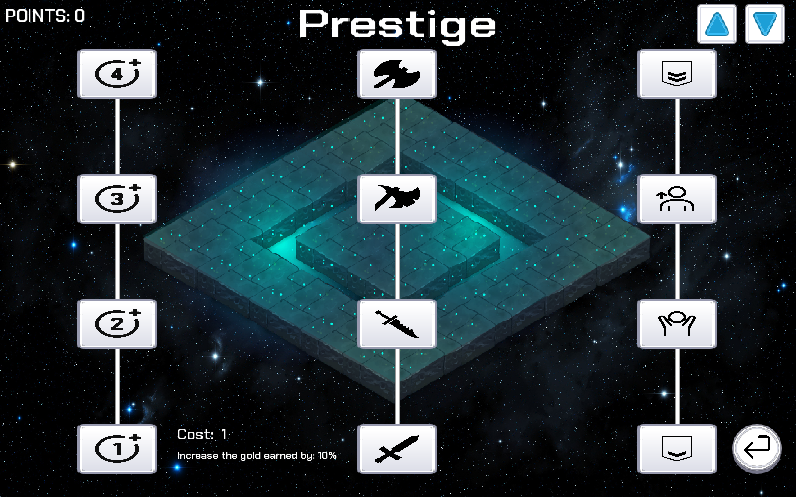
\includegraphics[width=12cm]{img/prestige_image.png} 
        \caption{Arbre de compétence de prestige}
        \label{Arbre de compétence de prestige}
\end{figure}
\begin{figure}[h]
    \centering
    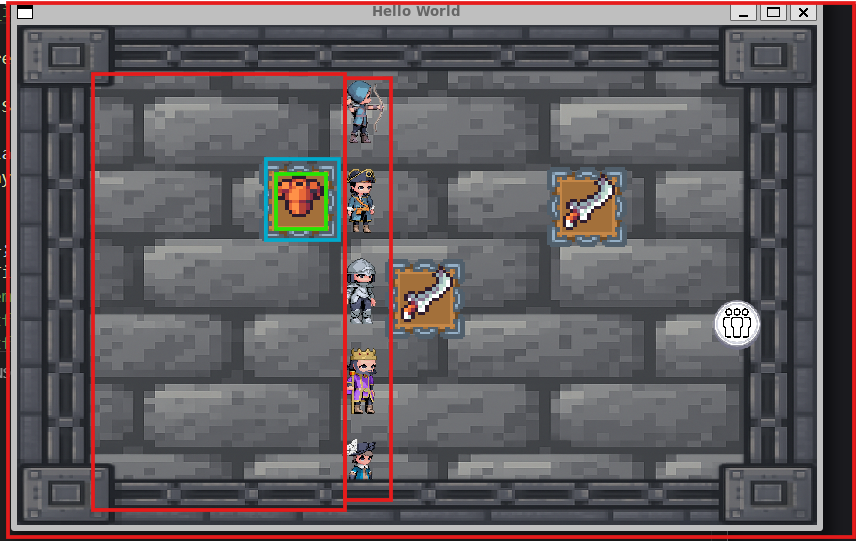
\includegraphics[width=12cm]{img/inv.png}
    \caption{Interface de l'inventaire avec les différents éléments visuels. Le carré rouge indique la zone de gestion des items et des interface scroll et les carrer vers les items .}
    \label{interface}
\end{figure}
\begin{figure}[h] 
    \centering 
    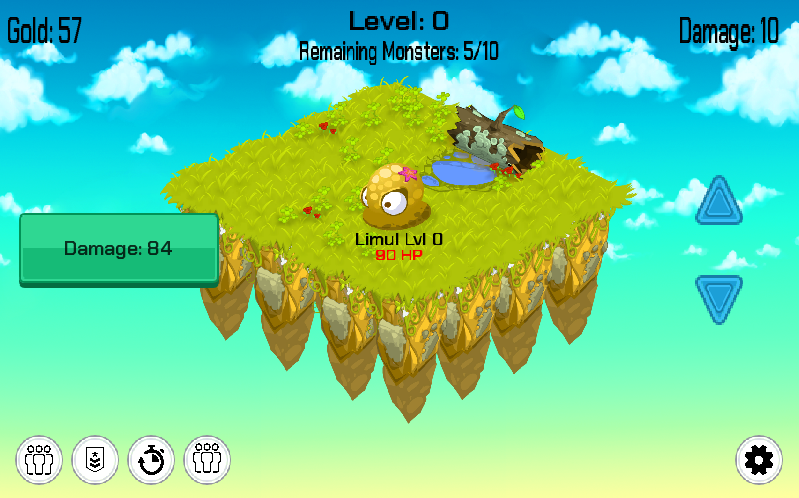
\includegraphics[width=12cm]{img/jeuPrincipale.png} 
    \caption{Menu principale}
\end{figure}
\begin{figure}[h] 
    \centering 
    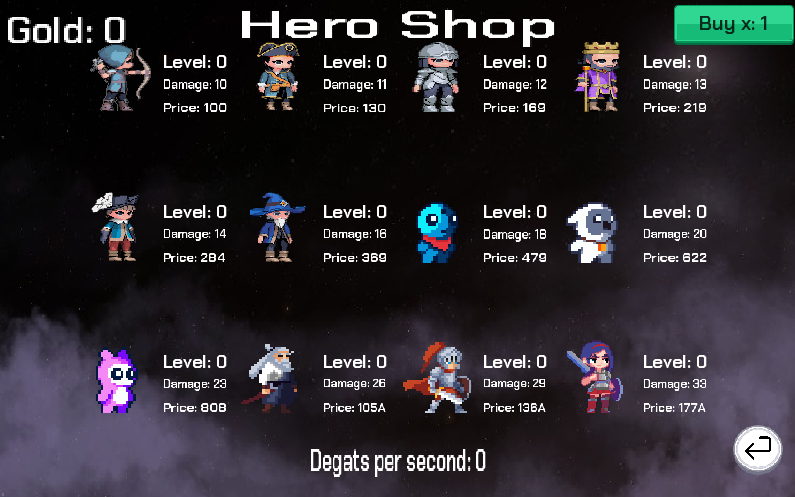
\includegraphics[width=12cm]{img/MenuHeros.png} 
    \caption{Menu des héros}
\end{figure}
\begin{figure}[h] 
    \centering 
    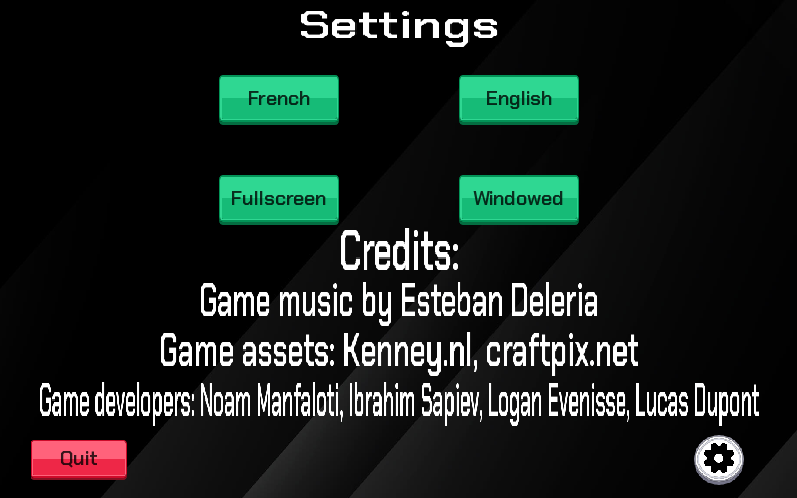
\includegraphics[width=12cm]{img/Parametre.png} 
    \caption{Menu des paramètres}
\end{figure}

\end{document}